\documentclass[11pt,a4paper]{article}

\usepackage[utf8]{inputenc}
\usepackage[T1]{fontenc}
\usepackage[spanish,es-noshorthands,es-tabla]{babel}
\usepackage{lmodern}
\usepackage{microtype}
\usepackage[margin=2.5cm]{geometry}
\usepackage{graphicx}
\usepackage{booktabs}
\usepackage{longtable}
\usepackage{array}
\usepackage{amsmath}
\usepackage{enumitem}
\usepackage{csquotes}
\usepackage[style=authoryear,backend=biber,maxcitenames=2,maxbibnames=10,uniquelist=false,uniquename=false]{biblatex}
\addbibresource{../referencias.bib}
\addbibresource{../referencias_geo.bib}
\addbibresource{../referencias_grupo_a.bib}
\addbibresource{../referencias_grupo_b.bib}
\addbibresource{../referencias_grupo_c.bib}
\addbibresource{../referencias_grupo_d.bib}
\addbibresource{../referencias_literatura.bib}

\usepackage{xurl}
\usepackage[hidelinks]{hyperref}

\DeclareFieldFormat{titlecase}{#1}
\setlength{\parskip}{0.35em}
\setlength{\emergencystretch}{2em}
\setcounter{biburlnumpenalty}{100}
\setcounter{biburllcpenalty}{100}
\setcounter{biburlucpenalty}{100}
\setlength{\parindent}{1.2em}
\setlist{itemsep=1pt,topsep=3pt}

% Generado por iica.exportar: no editar a mano.
\newcommand{\MXindice}{37{,}5}
\newcommand{\MXrango}{45}
\newcommand{\MXrangoBajo}{42}
\newcommand{\MXrangoAlto}{49}
\newcommand{\NPaises}{56}
\newcommand{\MXdimA}{42{,}8}
\newcommand{\MXdimB}{23{,}3}
\newcommand{\MXdimC}{56{,}9}
\newcommand{\MXdimD}{62{,}5}
\newcommand{\MXdimE}{31{,}7}
\newcommand{\MXdimF}{22{,}1}
\newcommand{\MXrangoAL}{12}
\newcommand{\NAL}{22}
\newcommand{\CHHindice}{45{,}7}
\newcommand{\CHHrango}{11}
\newcommand{\CHHrangoBajo}{7}
\newcommand{\CHHrangoAlto}{22}
\newcommand{\CHHdimA}{64{,}9}
\newcommand{\CHHdimB}{63{,}9}
\newcommand{\CHHdimC}{33{,}3}
\newcommand{\CHHdimD}{39{,}9}
\newcommand{\CHHdimE}{30{,}3}
\newcommand{\CHHdimF}{50{,}3}
\newcommand{\SONindice}{50{,}0}
\newcommand{\SONrango}{7}
\newcommand{\SONrangoBajo}{3}
\newcommand{\SONrangoAlto}{19}
\newcommand{\SONdimA}{72{,}3}
\newcommand{\SONdimB}{83{,}4}
\newcommand{\SONdimC}{44{,}4}
\newcommand{\SONdimD}{55{,}2}
\newcommand{\SONdimE}{24{,}2}
\newcommand{\SONdimF}{40{,}5}
\newcommand{\CDMXindice}{72{,}6}
\newcommand{\CDMXrango}{1}
\newcommand{\CDMXrangoBajo}{1}
\newcommand{\CDMXrangoAlto}{2}
\newcommand{\CDMXdimA}{97{,}3}
\newcommand{\CDMXdimB}{100{,}0}
\newcommand{\CDMXdimC}{48{,}3}
\newcommand{\CDMXdimD}{56{,}7}
\newcommand{\CDMXdimE}{53{,}7}
\newcommand{\CDMXdimF}{100{,}0}
\newcommand{\NACprimerAnio}{2020}
\newcommand{\NACprimerIndice}{33{,}2}
\newcommand{\NACultimoAnio}{2024}
\newcommand{\NACultimoIndice}{36{,}0}

% Generado por tablas.py: no editar a mano.
\newcommand{\NFuentesVerificadas}{28}
\newcommand{\NFuentesCandidatas}{4}
\newcommand{\NFuentesTotal}{33}
\newcommand{\NIndIntl}{16}
\newcommand{\NIndEst}{16}
\newcommand{\NIndNac}{14}
\newcommand{\NAbiertasVerif}{15}
\newcommand{\NNoRedistrib}{13}
\newcommand{\ALmedDimA}{51{,}9}
\newcommand{\OCDEmedDimA}{72{,}4}
\newcommand{\ALmedDimB}{37{,}8}
\newcommand{\OCDEmedDimB}{63{,}9}
\newcommand{\ALmedDimC}{56{,}7}
\newcommand{\OCDEmedDimC}{78{,}2}
\newcommand{\ALmedDimD}{51{,}2}
\newcommand{\OCDEmedDimD}{74{,}6}
\newcommand{\ALmedDimE}{36{,}2}
\newcommand{\OCDEmedDimE}{79{,}0}
\newcommand{\ALmedDimF}{14{,}8}
\newcommand{\OCDEmedDimF}{61{,}5}
\newcommand{\ALmedIndice}{38{,}2}
\newcommand{\OCDEmedIndice}{70{,}4}
\newcommand{\PrimerPais}{Suiza}
\newcommand{\PrimerPaisIndice}{87{,}9}
\newcommand{\UltimoPais}{Cuba}
\newcommand{\UltimoPaisIndice}{6{,}1}
\newcommand{\MXrangoOCDE}{37}
\newcommand{\NOCDE}{38}
\newcommand{\MXaritmetico}{39{,}9}
\newcommand{\PrimerAL}{Uruguay}
\newcommand{\PrimerALIndice}{65{,}2}
\newcommand{\CohWJP}{0{,}96}
\newcommand{\CohWGIvoz}{0{,}95}
\newcommand{\CohPartPres}{0{,}09}
\newcommand{\CohCorrup}{-0{,}04}
\newcommand{\CohConfianza}{0{,}30}
\newcommand{\NSubrepEst}{6}
\newcommand{\MaxRpobEst}{0{,}30}
\newcommand{\NWinsorEst}{6}
\newcommand{\NWinsorIntl}{0}
\newcommand{\NEnt}{32}
\newcommand{\UltimaEnt}{Chiapas}
\newcommand{\UltimaEntIndice}{12{,}7}
\newcommand{\SegundaEnt}{Querétaro}
\newcommand{\SegundaEntIndice}{56{,}7}
\newcommand{\MedEntIndice}{38{,}7}
\newcommand{\EntMedDimA}{60{,}9}
\newcommand{\EntMedDimB}{36{,}1}
\newcommand{\EntMedDimC}{43{,}2}
\newcommand{\EntMedDimD}{28{,}9}
\newcommand{\EntMedDimE}{49{,}8}
\newcommand{\EntMedDimF}{31{,}6}
\newcommand{\CHHaritmetico}{47{,}1}
\newcommand{\SONaritmetico}{53{,}3}
\newcommand{\NACDoneini}{41{,}8}
\newcommand{\NACDoneiniAnio}{2012}
\newcommand{\NACDonefin}{48{,}8}
\newcommand{\NACDonefinAnio}{2024}
\newcommand{\NACDtwoini}{26{,}9}
\newcommand{\NACDtwoiniAnio}{2020}
\newcommand{\NACDtwofin}{23{,}2}
\newcommand{\NACDtwofinAnio}{2025}
\newcommand{\NACDfourini}{51{,}1}
\newcommand{\NACDfouriniAnio}{2013}
\newcommand{\NACDfourfin}{62{,}7}
\newcommand{\NACDfourfinAnio}{2025}
\newcommand{\NACDfiveini}{37{,}8}
\newcommand{\NACDfiveiniAnio}{2012}
\newcommand{\NACDfivefin}{32{,}0}
\newcommand{\NACDfivefinAnio}{2025}
\newcommand{\NACDsixini}{4{,}8}
\newcommand{\NACDsixiniAnio}{2020}
\newcommand{\NACDsixfin}{17{,}7}
\newcommand{\NACDsixfinAnio}{2025}
\newcommand{\NACdesde}{2012}
\newcommand{\IDDanio}{2024}
\newcommand{\IDDchh}{3{,}17}
\newcommand{\IDDson}{5{,}24}
\newcommand{\RhoIDD}{0{,}68}


\title{\textbf{Hacia la medición de la Inteligencia Cívica Aumentada:\\
índices parciales con datos abiertos para México,\\ sus entidades federativas y la comparación internacional}}
\author{Ricardo Zenteno Fernández\thanks{Consejero Electoral, Instituto Estatal Electoral de Chihuahua. \texttt{rzentenof@ieechihuahua.org.mx}}
\and Julio Waissman Vilanova\thanks{Coordinador de la Maestría en Ciencia de Datos, Universidad de Sonora. \texttt{julio.waissman@unison.mx}}}
\date{Noviembre de 2026}

\begin{document}
\maketitle

\begin{abstract}
\noindent
El concepto de Inteligencia Cívica Aumentada (ICA) describe la capacidad emergente de un ecosistema democrático para comprender, deliberar, decidir, cocrear, actuar y aprender sobre problemas públicos mediante la interacción entre capacidades humanas, inteligencia colectiva, instituciones habilitadoras e inteligencia artificial, preservando la agencia humana. Su propuesta original deja la medición, el Índice de Inteligencia Cívica Aumentada (IICA), como agenda de investigación. Este artículo da un primer paso: construye tres índices parciales con datos abiertos, siguiendo la metodología de indicadores compuestos de la OCDE y el Centro Común de Investigación de la Comisión Europea. El índice internacional (IICA-I) compara a México en un panel de \NPaises{} países de América Latina y la OCDE; el nacional (IICA-N) sigue a México desde \NACdesde; y el estatal (IICA-E) compara las \NEnt{} entidades federativas, con énfasis en Chihuahua y Sonora. Se verificaron \NFuentesVerificadas{} fuentes descargándolas desde su origen. México obtiene \MXindice{} puntos sobre 100 y ocupa el lugar \MXrango{} (intervalo de sensibilidad \MXrangoBajo--\MXrangoAlto). En el nivel estatal, Sonora ocupa el lugar \SONrango{} y Chihuahua el \CHHrango. Los resultados deben leerse como índices de \emph{contexto}: los datos abiertos capturan sobre todo la capacidad instalada de los ecosistemas y casi nunca los resultados emergentes de los procesos de cocreación, que requieren mediciones propias.

\medskip
\noindent\textbf{Palabras clave:} inteligencia cívica, inteligencia artificial, indicadores compuestos, datos abiertos, democracia, entidades federativas.
\end{abstract}

\begin{otherlanguage}{english}
\begin{abstract}
\noindent
Augmented Civic Intelligence (ICA, in Spanish) is the emergent capacity of a democratic ecosystem to understand, deliberate, decide, co-create, act and learn about public problems through the interaction of human capacities, collective intelligence, enabling institutions and artificial intelligence, while preserving human agency. Its original proposal leaves measurement, the Augmented Civic Intelligence Index (IICA), as a research agenda. This article takes a first step by building three partial indices from open data, following the OECD and European Commission Joint Research Centre methodology for composite indicators. The international index compares Mexico within a panel of \NPaises{} Latin American and OECD countries; the national index follows Mexico since \NACdesde; and the state index compares Mexico's \NEnt{} states, with emphasis on Chihuahua and Sonora. \NFuentesVerificadas{} sources were verified by downloading them from their publishers. Mexico scores \MXindice{} out of 100 and ranks \MXrango{} (sensitivity interval \MXrangoBajo--\MXrangoAlto). Sonora ranks \SONrango{} and Chihuahua \CHHrango{} among the states. The results are \emph{context} indices: open data mostly capture the installed capacity of ecosystems and seldom the emergent outcomes of co-creation processes, which require their own measurement.

\medskip
\noindent\textbf{Keywords:} civic intelligence, artificial intelligence, composite indicators, open data, democracy, Mexican states.
\end{abstract}
\end{otherlanguage}

%=====================================================================
\section{Introducción}
%=====================================================================

La expansión de la inteligencia artificial (IA) no solo cambia los instrumentos de participación pública: también interviene en las capacidades cognitivas con las que las personas analizan información, generan alternativas y construyen conocimiento. A partir de esa constatación, \textcite{zenteno_ica_2026} propone el concepto de \emph{Inteligencia Cívica Aumentada} (ICA) como una propiedad emergente de un ecosistema democrático institucional y social, formula un modelo explicativo (MICA), lo ilustra con el Hackathón de Ciberdemocracia de Chihuahua y plantea, como agenda futura, un Índice de Inteligencia Cívica Aumentada (IICA).

Una revisión documental previa encontró que ningún índice existente mide a la vez capacidades cívicas, inteligencia colectiva e integración ética de la IA dentro de procesos democráticos, a escala de institución o comunidad, ni distingue entre capacidad instalada, activación y resultados emergentes \parencite{informe_ica_2026}. Esa misma revisión identificó una ruta metodológica: el \emph{Handbook on Constructing Composite Indicators} de la OCDE y el Centro Común de Investigación (JRC) de la Comisión Europea \parencite{ocde_jrc_2008,jrc_coin_2019}.

Este artículo aborda una pregunta acotada: \emph{¿qué parte del IICA puede aproximarse hoy con datos abiertos o existentes, y qué muestra esa aproximación para México, para sus entidades federativas y en la comparación internacional?} La respuesta tiene dos componentes. El primero es un inventario verificado de fuentes y de lo que cada una puede y no puede medir. El segundo son tres índices parciales ---internacional, nacional y estatal--- calculados con un \emph{pipeline} reproducible y publicados junto con su código.

Conviene adelantar la principal limitación. Los datos abiertos describen, sobre todo, la \emph{capacidad instalada} de un ecosistema: conectividad, instituciones, organizaciones, investigación. Rara vez describen la \emph{activación} de esas capacidades en procesos concretos de cocreación, y nunca sus \emph{resultados emergentes}, que son el núcleo del concepto. Por eso llamamos a estos índices \emph{IICA parciales de contexto}: describen las condiciones en las que la ICA puede o no emerger, no la ICA misma.

%=====================================================================
\section{El IICA y la brecha de medición}
%=====================================================================

\subsection{Concepto, modelo y dimensiones}

\textcite{zenteno_ica_2026} define la ICA como la propiedad emergente de un ecosistema democrático institucional y social que amplía la capacidad de una comunidad política para comprender problemas públicos, integrar conocimientos, deliberar, construir alternativas, decidir, coordinar acciones y aprender colectivamente, mediante la interacción ética y deliberada entre capacidades humanas, inteligencia colectiva, instituciones habilitadoras e IA, preservando la agencia humana, la pluralidad, la inclusión, la transparencia y la responsabilidad democrática.

La propuesta retoma dos tradiciones. De \textcite{engelbart_1962} toma la idea de \emph{aumentación}: incrementar la capacidad de las personas para abordar situaciones problemáticas complejas, sin sustituirlas. De \textcite{schuler_2001,schuler_2014} toma la \emph{inteligencia cívica}, entendida como la capacidad de las colectividades para abordar de forma equitativa y eficaz problemas compartidos, orientada al bien común. El Modelo de Inteligencia Cívica Aumentada (MICA) organiza estos elementos como un ecosistema adaptativo en el que las instituciones habilitadoras son un componente interno, distingue entre capacidad instalada y activación, y usa el valor público democrático \parencite{moore_1995} como criterio de validación \parencite{zenteno_ica_2026}.

Para el índice, la propuesta original define seis dimensiones preliminares \parencite{zenteno_ica_2026}:
\begin{enumerate}
  \item capacidades cívicas y humanas;
  \item inteligencia colectiva;
  \item integración ética de la IA;
  \item instituciones habilitadoras y cocreación;
  \item valor público democrático;
  \item continuidad y retroalimentación;
\end{enumerate}
más criterios transversales de agencia humana, pluralidad, inclusión, transparencia y rendición de cuentas. También advierte dos riesgos: reducir una propiedad compleja a una calificación simplificada y confundir capacidad tecnológica con capacidad democrática.

\subsection{Antecedentes cercanos}

La ICA dialoga con una literatura reciente que combina IA, inteligencia colectiva y democracia. \textcite{cui_yasseri_2024} conceptualizan la inteligencia colectiva aumentada por IA como un sistema multicapa en el que humanos e IA aportan capacidades complementarias, sin un objeto específicamente democrático. \textcite{deliddo_2026} proponen la inteligencia colectiva humano-IA para la democracia deliberativa (CI4DD), y el \emph{Handbook} editado por \textcite{pournaras_handbook_2026} dedica su primera parte a la inteligencia colectiva asistida por IA para la democracia. \textcite{schuler_ci4cg_2018} ya habían vinculado la inteligencia cívica con la inteligencia colectiva para el bien común. Con el término \emph{augmented democracy}, \textcite{hidalgo_2018} propuso gemelos digitales que amplíen la participación directa, y \textcite{pournaras_2020} usó la expresión en el contexto de ciudades inteligentes. Desde la práctica, la Habermas Machine mostró que un mediador basado en modelos de lenguaje puede ayudar a grupos a encontrar puntos de acuerdo \parencite{tessler_2024}.

\subsection{La brecha de medición}

En cuanto a la medición, el antecedente más cercano por su vocabulario es el índice de compromiso cívico de \textcite{nechesov_ruponen_2024}, pero mide la calidad de la participación en una plataforma, no las capacidades de un ecosistema. Los índices de democracia, gobierno digital o preparación para la IA miden países, no instituciones ni comunidades, y ninguno integra las seis dimensiones \parencite{informe_ica_2026}. Entre los marcos útiles para el diseño están las directrices de evaluación de procesos deliberativos de la OCDE \parencite{ocde_evaluacion_2021}, el modelo de madurez de la e-participación de \textcite{serdult_2023} y el Índice Global de IA Responsable, que penaliza de forma no compensatoria los usos inaceptables de IA \parencite{girai_metodo_2026}.

Este trabajo no pretende cerrar esa brecha. Su objetivo es más modesto: hacer explícito qué partes del IICA pueden medirse con información pública y cuáles requieren instrumentos nuevos.

%=====================================================================
\section{Datos y método}
%=====================================================================

\subsection{Tres niveles de análisis}

\begin{itemize}
  \item \textbf{IICA-I (internacional).} Compara a México con los países de América Latina y el Caribe y los miembros de la OCDE (\NPaises{} países con dato en todas las dimensiones). Para cada indicador se usa el año más reciente que cubra al menos el 70\,\% de los países.
  \item \textbf{IICA-N (nacional).} Sigue a México desde \NACdesde{} con los indicadores internacionales que tienen serie histórica.
  \item \textbf{IICA-E (estatal).} Compara las \NEnt{} entidades federativas con fuentes nacionales que publican datos por entidad. Para cada indicador se usa el año más reciente con las \NEnt{} entidades.
\end{itemize}

\subsection{Inventario y selección de fuentes}

Se revisaron \NFuentesTotal{} fuentes candidatas. Una fuente solo se aceptó si su archivo pudo descargarse desde el origen y si el valor de México, o de las entidades, pudo leerse y contrastarse con cifras publicadas por el propio editor. Con este criterio se verificaron \NFuentesVerificadas{} fuentes, todas con descarga automática; \NFuentesCandidatas{} quedaron pendientes porque requieren registro o navegador (LAPOP, Latinobarómetro, LATINNO y la Alianza para el Gobierno Abierto) \parencite{lapop_americasbarometer,latinobarometro2026,pogrebinschi_latinno2021,ogp_datos}. La Encuesta Nacional de Cultura Cívica 2020 se descartó para el nivel estatal porque solo es representativa por región \parencite{inegi_encuci_2020}.

La selección de indicadores siguió cinco criterios:
\begin{enumerate}
  \item entre dos y tres indicadores por dimensión;
  \item no combinar el total de una fuente con sus propios componentes, ni indicadores construidos con los mismos datos;
  \item preferir fuentes con licencia abierta;
  \item expresar los conteos absolutos como tasas por 100 mil habitantes, con la población del Banco Mundial \parencite{bancomundial_wdi} o de CONAPO \parencite{conapo_proyecciones_2023};
  \item clasificar cada indicador por dimensión, por capa (capacidad instalada, activación o resultado) y por sentido (si más es mejor o peor).
\end{enumerate}
Los cuadros \ref{tab:ind-intl} y \ref{tab:ind-est} listan los \NIndIntl{} indicadores internacionales y los \NIndEst{} estatales, con su fuente, el año utilizado y los valores en su escala original. El IICA-N usa \NIndNac{} de los indicadores internacionales.

{\footnotesize
\begin{longtable}{@{}p{0.4cm}>{\raggedright\arraybackslash}p{6.25cm}>{\raggedright\arraybackslash}p{1.8cm}p{0.7cm}r@{}}
\caption{Indicadores del IICA-I (internacional), año utilizado y valor de México en su escala original. ($-$): menor es mejor. Los conteos se expresan por 100 mil habitantes. Fuentes: \parencite{bancomundial_wdi,dsp_v8,girai2026,github_innovationgraph,undesa_egov2024,vdem_v16,wipo_gii2026,wjp_rolindex2026}.}\label{tab:ind-intl}\\
\toprule
D. & Indicador & Fuente & Año & México\\
\midrule
\endfirsthead
\toprule
D. & Indicador & Fuente & Año & México\\
\midrule
\endhead
\bottomrule
\endfoot
1 & Personas que usan internet (\% de la población) & Banco Mundial & 2024 & 83{,}1\\
1 & Matrícula en educación terciaria (\% bruto) & Banco Mundial & 2023 & 47{,}5\\
1 & Índice del componente deliberativo (v2xdl\_delib) & V-Dem v16 & 2025 & 0{,}43\\
2 & Índice de participación de la sociedad civil (v2x\_cspart) & V-Dem v16 & 2025 & 0{,}49\\
2 & Colaboración con otras economías en GitHub (suma anual) [por 100 mil hab.] & GitHub IG & 2025 & 189{,}1\\
3 & Puntaje GIRAI (global) & GIRAI 2026 & 2026 & 27{,}9\\
3 & Contenido de la protección legal de la privacidad (v2smprivcon) & DSP v8 & 2025 & 0{,}81\\
3 & Índice de Servicios en Línea (OSI) & ONU E-Gov & 2024 & 0{,}76\\
4 & Índice del componente participativo (v2x\_partip) & V-Dem v16 & 2025 & 0{,}65\\
4 & Factor 3: Gobierno abierto & WJP & 2026 & 0{,}54\\
4 & Índice de E-Participación (EPI) & ONU E-Gov & 2024 & 0{,}74\\
5 & Voz y rendición de cuentas (WGI) & Banco Mundial & 2025 & -0{,}28\\
5 & Control de la corrupción (WGI) & Banco Mundial & 2025 & -0{,}94\\
5 & Índice del componente igualitario (v2x\_egal) & V-Dem v16 & 2025 & 0{,}47\\
6 & Global Innovation Index (puntaje) & GII (OMPI) & 2026 & 30{,}6\\
6 & Cuentas de desarrolladores en GitHub (al cierre del 4.º trimestre) [por 100 mil hab.] & GitHub IG & 2025 & 1\,999\\
\end{longtable}
}

{\footnotesize
\begin{longtable}{@{}p{0.4cm}>{\raggedright\arraybackslash}p{4.75cm}>{\raggedright\arraybackslash}p{1.8cm}p{0.7cm}rrr@{}}
\caption{Indicadores del IICA-E (estatal), año utilizado y valores nacional, de Chihuahua y de Sonora en su escala original (s.\,d.: sin dato publicado en ese nivel). Fuentes: \parencite{anuies_anuario_2025,bienestar_rfosc_2025,impi_cifras_2026,inai_cide_mga_2021,ine_computos_2024,inegi_cnge_2025,inegi_denue_2026,inegi_encig_2025,inegi_endutih_2025,secihti_snii_2025}.}\label{tab:ind-est}\\
\toprule
D. & Indicador & Fuente & Año & Nacional & Chih. & Son.\\
\midrule
\endfirsthead
\toprule
D. & Indicador & Fuente & Año & Nacional & Chih. & Son.\\
\midrule
\endhead
\bottomrule
\endfoot
1 & Personas usuarias de internet (\% de la población de 6 años y más) & ENDUTIH & 2025 & 86{,}1 & 88{,}8 & 88{,}8\\
1 & Hogares que disponen de computadora (\%) & ENDUTIH & 2025 & 44{,}7 & 48{,}6 & 49{,}6\\
1 & Matrícula total de educación superior (TSU, licenciatura, normal y posgrado; todas las modalidades) [por 100 mil hab.] & ANUIES & 2025 & 4\,319 & 3\,812 & 4\,440\\
2 & OSC con CLUNI en estatus ACTIVA [por 100 mil hab.] & Reg. Fed. OSC & 2025 & 4{,}9 & 5{,}9 & 7{,}5\\
3 & Personas usuarias de internet que lo usan para interactuar con el gobierno (\%) & ENDUTIH & 2025 & 35{,}7 & 33{,}4 & 32{,}0\\
3 & Tipos de trámite o servicio que se pueden presentar por medios electrónicos (de 24) & CNGE & 2025 & s.\,d. & 11{,}0 & 11{,}0\\
3 & Tipos de trámite o servicio con servicio web transaccional (de 24) & CNGE & 2025 & s.\,d. & 1{,}0 & 6{,}0\\
4 & Índice de Gobierno Abierto (MGA) & MGA & 2021 & 0{,}48 & 0{,}52 & 0{,}52\\
4 & Espacios de participación con nivel de incidencia de deliberación o cogestión (número) [por 100 mil hab.] & CNGE & 2025 & 0{,}55 & 0{,}57 & 1{,}05\\
4 & Solicitudes de acceso a la información recibidas por la Administración Pública estatal (número) [por 100 mil hab.] & CNGE & 2025 & 257{,}9 & 193{,}8 & 298{,}3\\
5 & Participación ciudadana, elección de Presidencia (votos totales / lista nominal) & INE & 2024 & 61{,}0 & 53{,}2 & 51{,}1\\
5 & Tasa de prevalencia de corrupción en trámites (víctimas por cada 100 000 habitantes) ($-$) & ENCIG & 2025 & 15\,642 & 18\,420 & 18\,355\\
5 & Población que confía mucho o algo en el gobierno estatal (\%) & ENCIG & 2025 & 40{,}4 & 41{,}5 & 37{,}8\\
6 & Personas investigadoras con reconocimiento vigente en el SNII [por 100 mil hab.] & SNII & 2025 & 33{,}6 & 26{,}2 & 39{,}0\\
6 & Establecimientos en la rama SCIAN 5415 (servicios de diseño de sistemas de cómputo y servicios relacionados) [por 100 mil hab.] & DENUE & 2026 & 2{,}3 & 1{,}9 & 3{,}1\\
6 & Solicitudes de patente de mexicanos por entidad federativa del solicitante [por 100 mil hab.] & IMPI & 2025 & 0{,}86 & 1{,}41 & 0{,}51\\
\end{longtable}
}


El cuadro \ref{tab:cobertura} resume la cobertura por dimensión y capa. Ningún nivel tiene indicadores de resultados emergentes, y en el nivel estatal la dimensión de inteligencia colectiva descansa en un solo indicador.

\begin{table}[htbp]\centering\footnotesize
\caption{Cobertura: número de indicadores por dimensión, capa y nivel. Ningún nivel tiene indicadores de resultados emergentes; las celdas vacías no se imputan.}\label{tab:cobertura}
\begin{tabular}{@{}p{5.2cm}cccccc c@{}}
\toprule
 & \multicolumn{3}{c}{IICA-I} & \multicolumn{3}{c}{IICA-E} & IICA-N\\
\cmidrule(lr){2-4}\cmidrule(lr){5-7}
Dimensión & Inst. & Activ. & Result. & Inst. & Activ. & Result. & Total\\
\midrule
1. Capacidades cívicas y humanas & 2 & 1 & \textemdash & 3 & \textemdash & \textemdash & 3\\
2. Inteligencia colectiva & \textemdash & 2 & \textemdash & 1 & \textemdash & \textemdash & 2\\
3. Integración ética de la IA y gobierno digital & 3 & \textemdash & \textemdash & 2 & 1 & \textemdash & 2\\
4. Instituciones habilitadoras y cocreación & 2 & 1 & \textemdash & 1 & 2 & \textemdash & 3\\
5. Valor público democrático & 2 & \textemdash & 1 & \textemdash & 1 & 2 & 3\\
6. Continuidad y retroalimentación & \textemdash & 1 & 1 & 2 & \textemdash & 1 & 1\\
\bottomrule
\end{tabular}
\end{table}


\subsection{Construcción de los índices}

La metodología sigue el Manual OCDE/JRC \parencite{ocde_jrc_2008} y la guía del JRC-COIN \parencite{jrc_coin_2019}.

\paragraph{Valores atípicos.} En los índices de corte transversal (IICA-I e IICA-E) se aplica la regla del JRC-COIN: si un indicador tiene asimetría mayor que 2 en valor absoluto y curtosis mayor que 3,5, se winsorizan sus valores extremos, uno a la vez y hasta un máximo de cinco, hasta que deja de cumplir la regla. Se winsorizaron \NWinsorEst{} indicadores estatales y \NWinsorIntl{} internacionales; en el nivel estatal, el caso típico es la Ciudad de México, que concentra registros federales como las organizaciones de la sociedad civil y las personas investigadoras.

\paragraph{Normalización.} Cada indicador $x$ se lleva a una escala de 0 a 100 con el método min-max,
\[
  z = 100\,\frac{x-\min(x)}{\max(x)-\min(x)},
\]
y se invierte ($100-z$) cuando más es peor, como en la prevalencia de corrupción.

\paragraph{Dimensiones.} El puntaje de cada dimensión es el promedio simple de sus indicadores normalizados. Los pesos se asignan por dimensión, no por indicador, para que las dimensiones con más indicadores no pesen más \parencite{ocde_jrc_2008}.

\paragraph{Agregación.} El índice es la media geométrica de las seis dimensiones con pesos iguales. Se eligió la media geométrica porque es menos compensatoria que la aritmética: un puntaje alto en una dimensión no compensa por completo uno bajo en otra, lo que es coherente con la idea de que la capacidad tecnológica no debe sustituir a la democrática \parencite{zenteno_ica_2026,ocde_jrc_2008}. Para evitar que un cero anule el producto, dentro de la media geométrica los puntajes se reescalan de $[0,100]$ a $[1,100]$.

\paragraph{Sensibilidad.} Se recalcula el índice 1\,000 veces con pesos aleatorios (distribución de Dirichlet) y con ambas fórmulas de agregación, aritmética y geométrica. Para cada unidad se reporta el intervalo de su lugar entre los percentiles 5 y 95.

\paragraph{Coherencia.} Se calcula la correlación de cada indicador normalizado con su dimensión y con el índice, y se marcan las alertas del JRC-COIN \parencite{jrc_coin_2019}:
\begin{itemize}
  \item correlación con el índice mayor que 0,95: el indicador domina el índice;
  \item correlación entre $-0{,}3$ y $0{,}3$: el indicador está subrepresentado;
  \item en el nivel estatal, correlación con la población mayor que 0,6: sesgo de tamaño.
\end{itemize}

\paragraph{Serie nacional.} Para que el IICA-N sea comparable en el tiempo, los límites de la normalización se fijan con todo el panel de países de comparación en el periodo completo, previo tratamiento de atípicos. Además, una dimensión solo se calcula en los años en que todos sus indicadores tienen dato; así la composición de cada dimensión es constante. Las series bienales de la ONU \parencite{undesa_egov2024} se arrastran un año para cubrir los años sin edición. El índice agregado solo se calcula en los años en que las seis dimensiones tienen dato.

\paragraph{Reproducibilidad.} Todo el proceso ---descarga, procesamiento, cálculo y exportación de cuadros, figuras y cifras de este artículo--- se ejecuta con un \emph{pipeline} en Python. Cada descarga guarda la fecha de acceso y la huella SHA-256 de los archivos. Ninguna cifra del texto se transcribió a mano.

%=====================================================================
\section{Resultados}
%=====================================================================

\subsection{México en la comparación internacional}

México obtiene un IICA-I de \MXindice{} puntos sobre 100 y ocupa el lugar \MXrango{} de \NPaises{} países (figura~\ref{fig:ranking-intl}). Con otras ponderaciones y con agregación aritmética (\MXaritmetico{} puntos), su lugar se mueve entre el \MXrangoBajo{} y el \MXrangoAlto. Entre los \NAL{} países de América Latina y el Caribe ocupa el lugar \MXrangoAL, y entre los \NOCDE{} miembros de la OCDE, el \MXrangoOCDE. La mediana del índice es de \ALmedIndice{} en América Latina y de \OCDEmedIndice{} en la OCDE. El primer lugar corresponde a \PrimerPais{} (\PrimerPaisIndice) y, en la región, a \PrimerAL{} (\PrimerALIndice).

\begin{figure}[htbp]
  \centering
  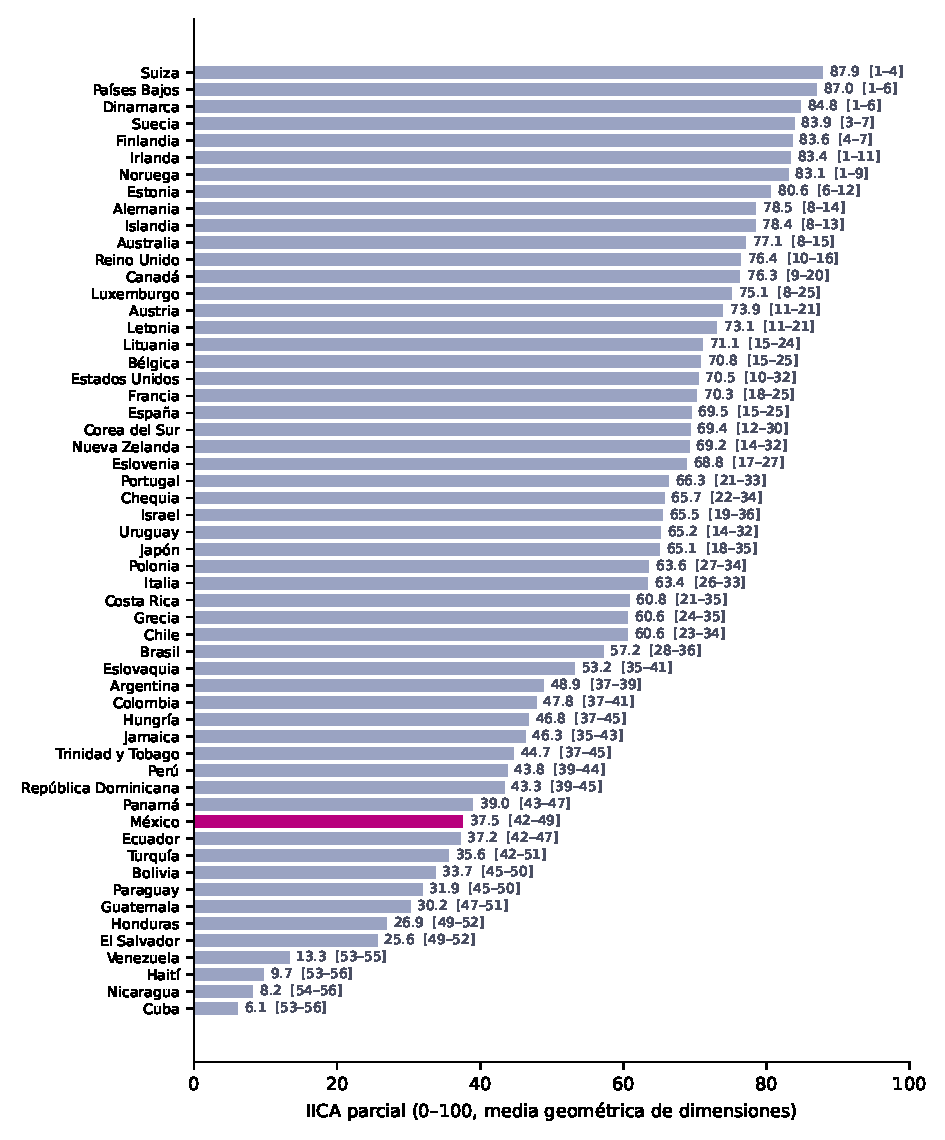
\includegraphics[width=\linewidth]{figuras/ranking_internacional.pdf}
  \caption{IICA-I por país (media geométrica de las seis dimensiones). Entre corchetes, el intervalo de lugares p5--p95 del análisis de sensibilidad. México, resaltado. Elaboración propia con las fuentes del cuadro~\ref{tab:ind-intl}.}
  \label{fig:ranking-intl}
\end{figure}

El perfil por dimensión (figura~\ref{fig:perfil-mx}) es desigual. Las dimensiones relativamente más fuertes de México son instituciones habilitadoras (\MXdimD) e integración ética de la IA y gobierno digital (\MXdimC), ambas por encima de la mediana latinoamericana (\ALmedDimD{} y \ALmedDimC). Las más débiles son continuidad y retroalimentación (\MXdimF), inteligencia colectiva (\MXdimB) y valor público democrático (\MXdimE). En inteligencia colectiva y valor público, México queda por debajo de la mediana de América Latina (\ALmedDimB{} y \ALmedDimE). En capacidades cívicas y humanas obtiene \MXdimA, frente a \ALmedDimA{} en la región y \OCDEmedDimA{} en la OCDE.

\begin{figure}[htbp]
  \centering
  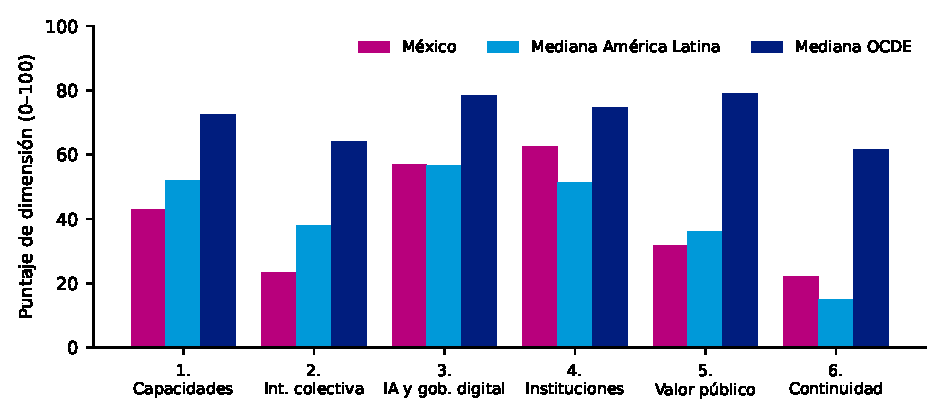
\includegraphics[width=\linewidth]{figuras/perfil_mexico.pdf}
  \caption{Puntajes por dimensión de México frente a las medianas de América Latina y de la OCDE (IICA-I). Elaboración propia.}
  \label{fig:perfil-mx}
\end{figure}

\subsection{México en el tiempo}

El IICA-N completo solo puede calcularse desde \NACprimerAnio, porque los indicadores de GitHub, que alimentan las dimensiones de inteligencia colectiva y de continuidad, empiezan ese año \parencite{github_innovationgraph}. Entre \NACprimerAnio{} y \NACultimoAnio{} el índice pasa de \NACprimerIndice{} a \NACultimoIndice{} puntos (figura~\ref{fig:serie}).

Por dimensión, las capacidades cívicas y humanas suben de \NACDoneini{} en \NACDoneiniAnio{} a \NACDonefin{} en \NACDonefinAnio{}, y las instituciones habilitadoras de \NACDfourini{} en \NACDfouriniAnio{} a \NACDfourfin{} en \NACDfourfinAnio. En cambio, el valor público democrático baja de \NACDfiveini{} en \NACDfiveiniAnio{} a \NACDfivefin{} en \NACDfivefinAnio. La continuidad y retroalimentación crece de \NACDsixini{} a \NACDsixfin{} entre \NACDsixiniAnio{} y \NACDsixfinAnio, pero desde niveles muy bajos. Estas variaciones deben leerse con cautela: son puntajes relativos al rango observado en el panel de comparación, de modo que un cambio puede reflejar tanto la evolución de México como la de los límites del panel.

\begin{figure}[htbp]
  \centering
  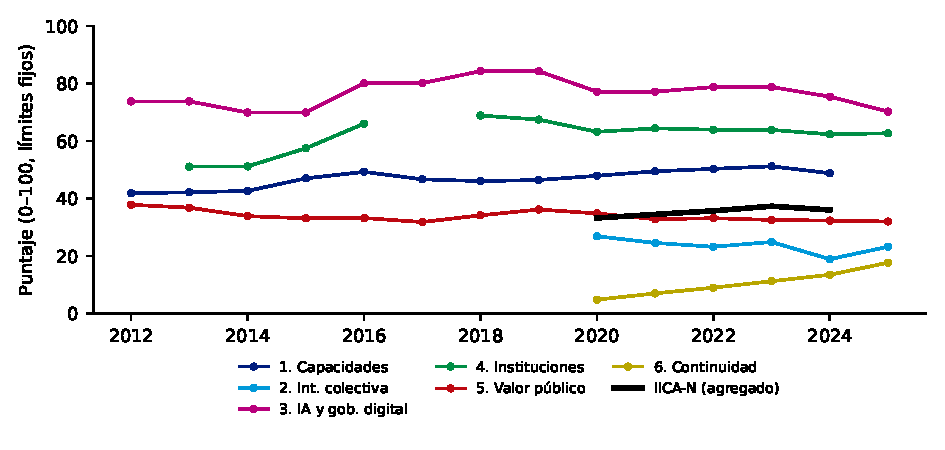
\includegraphics[width=\linewidth]{figuras/serie_nacional.pdf}
  \caption{IICA-N: puntajes por dimensión de México con límites de normalización fijos. Cada dimensión aparece solo en los años en que todos sus indicadores tienen dato; el índice agregado, solo cuando las seis dimensiones lo tienen. Elaboración propia.}
  \label{fig:serie}
\end{figure}

\subsection{Las entidades federativas}

El cuadro~\ref{tab:entidades} y la figura~\ref{fig:ranking-est} presentan el IICA-E. La Ciudad de México ocupa el primer lugar (\CDMXindice{} puntos; intervalo \CDMXrangoBajo--\CDMXrangoAlto), seguida de \SegundaEnt{} (\SegundaEntIndice). El último lugar corresponde a \UltimaEnt{} (\UltimaEntIndice). La mediana de las entidades es de \MedEntIndice{} puntos.

\begin{figure}[htbp]
  \centering
  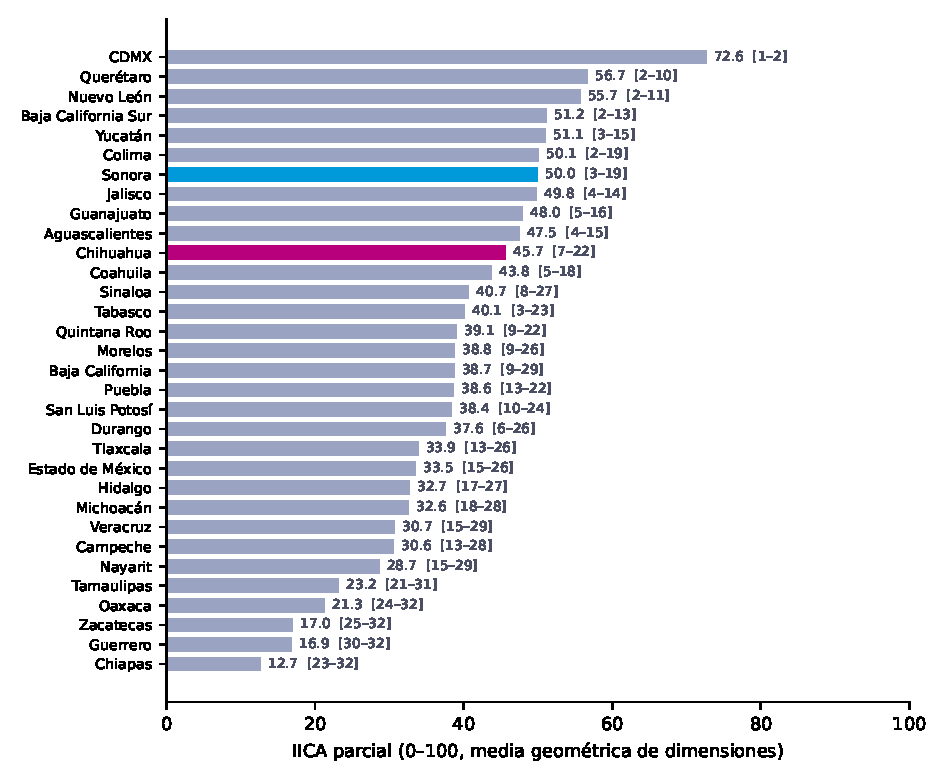
\includegraphics[width=0.92\linewidth]{figuras/ranking_estatal.pdf}
  \caption{IICA-E por entidad federativa, con el intervalo de lugares p5--p95 entre corchetes. Chihuahua (magenta) y Sonora (cian), resaltados. Elaboración propia con las fuentes del cuadro~\ref{tab:ind-est}.}
  \label{fig:ranking-est}
\end{figure}

{\scriptsize
\begin{longtable}{@{}rp{4.2cm}rcrrrrrr@{}}
\caption{IICA-E por entidad federativa: índice (media geométrica), intervalo de rangos p5--p95 del análisis de sensibilidad y puntajes por dimensión (0--100).}\label{tab:entidades}\\
\toprule
Lugar & Entidad & IICA-E & Rango p5--p95 & D1 & D2 & D3 & D4 & D5 & D6\\
\midrule
\endfirsthead
\toprule
Lugar & Entidad & IICA-E & Rango p5--p95 & D1 & D2 & D3 & D4 & D5 & D6\\
\midrule
\endhead
\bottomrule
\endfoot
1 & Ciudad de México & 72{,}6 & 1--2 & 97{,}3 & 100{,}0 & 48{,}3 & 56{,}7 & 53{,}7 & 100{,}0\\
2 & Querétaro & 56{,}7 & 2--10 & 76{,}8 & 73{,}8 & 56{,}5 & 20{,}0 & 75{,}2 & 64{,}9\\
3 & Nuevo León & 55{,}7 & 2--11 & 92{,}4 & 31{,}7 & 58{,}4 & 47{,}6 & 57{,}5 & 60{,}4\\
4 & Baja California Sur & 51{,}2 & 2--13 & 64{,}6 & 64{,}3 & 47{,}9 & 63{,}6 & 38{,}6 & 34{,}6\\
5 & Yucatán & 51{,}1 & 3--15 & 53{,}3 & 69{,}4 & 66{,}4 & 20{,}1 & 67{,}9 & 49{,}1\\
6 & Colima & 50{,}1 & 2--19 & 73{,}2 & 100{,}0 & 20{,}9 & 28{,}9 & 61{,}4 & 53{,}9\\
7 & \textbf{Sonora} & 50{,}0 & 3--19 & 72{,}3 & 83{,}4 & 44{,}4 & 55{,}2 & 24{,}2 & 40{,}5\\
8 & Jalisco & 49{,}8 & 4--14 & 64{,}7 & 49{,}9 & 32{,}9 & 49{,}8 & 46{,}3 & 58{,}8\\
9 & Guanajuato & 48{,}0 & 5--16 & 50{,}0 & 51{,}8 & 55{,}8 & 50{,}0 & 53{,}0 & 29{,}8\\
10 & Aguascalientes & 47{,}5 & 4--15 & 83{,}0 & 29{,}7 & 42{,}0 & 39{,}5 & 59{,}1 & 44{,}0\\
11 & \textbf{Chihuahua} & 45{,}7 & 7--22 & 64{,}9 & 63{,}9 & 33{,}3 & 39{,}9 & 30{,}3 & 50{,}3\\
12 & Coahuila de Zaragoza & 43{,}8 & 5--18 & 68{,}2 & 35{,}0 & 33{,}7 & 25{,}3 & 72{,}5 & 43{,}8\\
13 & Sinaloa & 40{,}7 & 8--27 & 76{,}7 & 40{,}7 & 47{,}0 & 31{,}2 & 18{,}3 & 49{,}1\\
14 & Tabasco & 40{,}1 & 3--23 & 62{,}7 & 17{,}5 & 72{,}2 & 58{,}8 & 51{,}9 & 15{,}2\\
15 & Quintana Roo & 39{,}1 & 9--22 & 57{,}2 & 37{,}6 & 59{,}4 & 36{,}5 & 38{,}1 & 18{,}0\\
16 & Morelos & 38{,}8 & 9--26 & 53{,}3 & 50{,}0 & 22{,}4 & 17{,}3 & 54{,}2 & 54{,}0\\
17 & Baja California & 38{,}7 & 9--29 & 79{,}5 & 59{,}4 & 26{,}1 & 37{,}9 & 18{,}2 & 35{,}4\\
18 & Puebla & 38{,}6 & 13--22 & 62{,}4 & 27{,}7 & 39{,}7 & 22{,}7 & 48{,}1 & 39{,}9\\
19 & San Luis Potosí & 38{,}4 & 10--24 & 44{,}9 & 20{,}1 & 53{,}4 & 35{,}9 & 49{,}9 & 33{,}4\\
20 & Durango & 37{,}6 & 6--26 & 54{,}1 & 87{,}7 & 31{,}7 & 24{,}9 & 41{,}6 & 16{,}0\\
21 & Tlaxcala & 33{,}9 & 13--26 & 43{,}0 & 37{,}1 & 35{,}8 & 20{,}7 & 63{,}2 & 17{,}6\\
22 & México & 33{,}5 & 15--26 & 55{,}1 & 29{,}9 & 54{,}8 & 19{,}2 & 42{,}7 & 16{,}6\\
23 & Hidalgo & 32{,}7 & 17--27 & 52{,}9 & 13{,}0 & 48{,}1 & 32{,}7 & 38{,}9 & 25{,}1\\
24 & Michoacán de Ocampo & 32{,}6 & 18--28 & 40{,}4 & 20{,}0 & 51{,}3 & 28{,}9 & 35{,}0 & 25{,}1\\
25 & Veracruz de Ignacio de la Llave & 30{,}7 & 15--29 & 37{,}6 & 28{,}7 & 59{,}7 & 14{,}8 & 49{,}8 & 14{,}9\\
26 & Campeche & 30{,}6 & 13--28 & 62{,}3 & 11{,}4 & 26{,}6 & 27{,}9 & 63{,}6 & 20{,}6\\
27 & Nayarit & 28{,}7 & 15--29 & 59{,}6 & 8{,}6 & 36{,}0 & 34{,}2 & 57{,}4 & 12{,}3\\
28 & Tamaulipas & 23{,}2 & 21--31 & 64{,}4 & 12{,}3 & 10{,}9 & 16{,}2 & 56{,}8 & 15{,}0\\
29 & Oaxaca & 21{,}3 & 24--32 & 18{,}1 & 46{,}4 & 25{,}1 & 7{,}7 & 28{,}0 & 15{,}9\\
30 & Zacatecas & 17{,}0 & 25--32 & 45{,}1 & 0{,}0 & 14{,}5 & 28{,}1 & 44{,}6 & 25{,}9\\
31 & Guerrero & 16{,}9 & 30--32 & 21{,}7 & 16{,}5 & 28{,}7 & 9{,}6 & 34{,}1 & 4{,}6\\
32 & Chiapas & 12{,}7 & 23--32 & 0{,}0 & 22{,}5 & 48{,}0 & 17{,}2 & 59{,}1 & 2{,}4\\
\end{longtable}
}


Los intervalos de sensibilidad son amplios en la parte media de la tabla. Muchas entidades no pueden distinguirse con seguridad, y las posiciones deben leerse como grupos más que como un orden estricto.

\paragraph{Sonora.} Sonora ocupa el lugar \SONrango{} con \SONindice{} puntos (intervalo \SONrangoBajo--\SONrangoAlto). Sus fortalezas relativas son la inteligencia colectiva (\SONdimB, frente a una mediana estatal de \EntMedDimB), medida por las organizaciones de la sociedad civil activas por habitante \parencite{bienestar_rfosc_2025}; las capacidades cívicas y humanas (\SONdimA); y las instituciones habilitadoras (\SONdimD, frente a \EntMedDimD). Su debilidad más marcada es el valor público democrático (\SONdimE, frente a una mediana de \EntMedDimE), que combina participación electoral, prevalencia de corrupción en trámites y confianza en el gobierno estatal \parencite{ine_computos_2024,inegi_encig_2025}.

\paragraph{Chihuahua.} Chihuahua ocupa el lugar \CHHrango{} con \CHHindice{} puntos (intervalo \CHHrangoBajo--\CHHrangoAlto). Destacan sus capacidades cívicas y humanas (\CHHdimA), su inteligencia colectiva (\CHHdimB) y su continuidad y retroalimentación (\CHHdimF, frente a una mediana de \EntMedDimF), en la que pesan las solicitudes de patente por habitante \parencite{impi_cifras_2026}. Sus dimensiones más débiles son el valor público democrático (\CHHdimE) y la integración de la IA y el gobierno digital (\CHHdimC, frente a \EntMedDimC): el gobierno estatal reporta pocos trámites con servicio transaccional en línea \parencite{inegi_cnge_2025}.

\paragraph{Lo que comparten.} Ambas entidades se ubican en la mitad superior del índice, pero las dos tienen su punto más débil en el valor público democrático. Las dos tienen una participación electoral por debajo de la nacional y una prevalencia de corrupción en trámites por encima de ella (cuadro~\ref{tab:ind-est}). La figura~\ref{fig:perfil-est} compara sus perfiles con la mediana de las entidades.

\begin{figure}[htbp]
  \centering
  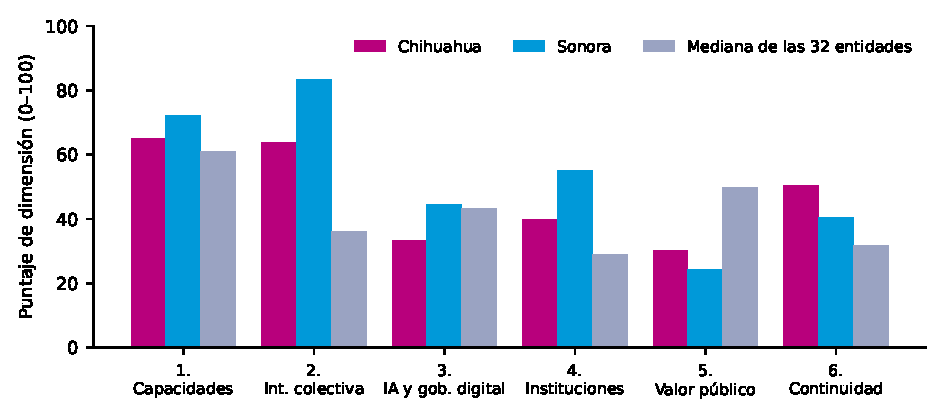
\includegraphics[width=\linewidth]{figuras/perfil_chihuahua_sonora.pdf}
  \caption{Puntajes por dimensión de Chihuahua y Sonora frente a la mediana de las 32 entidades (IICA-E). Elaboración propia.}
  \label{fig:perfil-est}
\end{figure}

\paragraph{Relación con otros índices.} Como referencia externa, la correlación de rangos de Spearman entre el IICA-E y el Índice de Desarrollo Democrático de México \parencite{iddmex_2024} de \IDDanio{} es de \RhoIDD. La relación es positiva pero lejos de ser perfecta, lo que sugiere que el IICA-E captura algo relacionado con el desarrollo democrático, pero no idéntico.

%=====================================================================
\section{Alcances y limitaciones}
%=====================================================================

\paragraph{Qué se mide.} Los índices miden sobre todo capacidad instalada y, en algunos indicadores, activación (cuadro~\ref{tab:cobertura}). Ningún indicador captura resultados emergentes. Por diseño, la ICA es una propiedad emergente de las interacciones dentro de un ecosistema \parencite{zenteno_ica_2026}; estos índices describen las condiciones de ese ecosistema, no la propiedad.

\paragraph{Coherencia estadística.} En el IICA-I, el factor de Gobierno abierto del WJP \parencite{wjp_rolindex2026} y el indicador de Voz y rendición de cuentas de los WGI \parencite{bancomundial_wdi} tienen correlaciones con el índice de \CohWJP{} y \CohWGIvoz, en el umbral en que un indicador empieza a dominar (cuadro~\ref{tab:coh-intl}). En el IICA-E, \NSubrepEst{} indicadores quedan subrepresentados (cuadro~\ref{tab:coh-est}). Los de valor público son el caso más claro: la participación electoral, la prevalencia de corrupción y la confianza en el gobierno estatal tienen correlaciones con el índice de \CohPartPres, \CohCorrup{} y \CohConfianza. Esa dimensión mide algo distinto del resto, lo que justifica conservarla, pero también advierte que el índice agregado oculta tensiones entre dimensiones. Ningún indicador estatal supera el umbral de sesgo de tamaño: la correlación más alta con la población, en valor absoluto, es de \MaxRpobEst.

\begin{table}[htbp]\centering\scriptsize
\caption{Coherencia estadística del IICA-I: correlación de Pearson de cada indicador normalizado con su dimensión y con el índice. Alertas según los umbrales de JRC-COIN.}\label{tab:coh-intl}
\begin{tabular}{@{}p{0.4cm}>{\raggedright\arraybackslash}p{6.0cm}rr>{\raggedright\arraybackslash}p{2.6cm}@{}}
\toprule
D. & Indicador & $r$ dim. & $r$ índice & Alerta\\
\midrule
1 & Personas que usan internet (\% de la población) & 0{,}81 & 0{,}86 & \\
1 & Matrícula en educación terciaria (\% bruto) & 0{,}72 & 0{,}44 & \\
1 & Índice del componente deliberativo (v2xdl\_delib) & 0{,}84 & 0{,}80 & \\
2 & Índice de participación de la sociedad civil (v2x\_cspart) & 0{,}85 & 0{,}82 & \\
2 & Colaboración con otras economías en GitHub (suma anual) & 0{,}89 & 0{,}79 & \\
3 & Puntaje GIRAI (global) & 0{,}91 & 0{,}85 & \\
3 & Contenido de la protección legal de la privacidad (v2smprivcon) & 0{,}65 & 0{,}48 & \\
3 & Índice de Servicios en Línea (OSI) & 0{,}84 & 0{,}83 & \\
4 & Índice del componente participativo (v2x\_partip) & 0{,}84 & 0{,}71 & \\
4 & Factor 3: Gobierno abierto & 0{,}93 & 0{,}96 & domina el índice\\
4 & Índice de E-Participación (EPI) & 0{,}93 & 0{,}81 & \\
5 & Voz y rendición de cuentas (WGI) & 0{,}96 & 0{,}95 & domina el índice\\
5 & Control de la corrupción (WGI) & 0{,}96 & 0{,}94 & \\
5 & Índice del componente igualitario (v2x\_egal) & 0{,}94 & 0{,}84 & \\
6 & Global Innovation Index (puntaje) & 0{,}96 & 0{,}88 & \\
6 & Cuentas de desarrolladores en GitHub (al cierre del 4.º trimestre) & 0{,}96 & 0{,}90 & \\
\bottomrule
\end{tabular}
\end{table}

\begin{table}[htbp]\centering\scriptsize
\caption{Coherencia estadística del IICA-E. La última columna numérica es la correlación con la población (sesgo de tamaño si $r>0{,}6$).}\label{tab:coh-est}
\begin{tabular}{@{}p{0.4cm}>{\raggedright\arraybackslash}p{6.0cm}rrr>{\raggedright\arraybackslash}p{2.6cm}@{}}
\toprule
D. & Indicador & $r$ dim. & $r$ índice & $r$ pob. & Alerta\\
\midrule
1 & Personas usuarias de internet (\% de la población de 6 años y más) & 0{,}88 & 0{,}66 & -0{,}10 & \\
1 & Hogares que disponen de computadora (\%) & 0{,}93 & 0{,}84 & 0{,}02 & \\
1 & Matrícula total de educación superior (TSU, licenciatura, normal y posgrado; todas las modalidades) & 0{,}85 & 0{,}61 & -0{,}02 & \\
2 & OSC con CLUNI en estatus ACTIVA & 1{,}00 & 0{,}70 & -0{,}06 & \\
3 & Personas usuarias de internet que lo usan para interactuar con el gobierno (\%) & 0{,}25 & 0{,}38 & 0{,}27 & \\
3 & Tipos de trámite o servicio que se pueden presentar por medios electrónicos (de 24) & 0{,}77 & 0{,}25 & -0{,}01 & subrepresentado\\
3 & Tipos de trámite o servicio con servicio web transaccional (de 24) & 0{,}75 & 0{,}10 & 0{,}26 & subrepresentado\\
4 & Índice de Gobierno Abierto (MGA) & 0{,}55 & 0{,}49 & 0{,}07 & \\
4 & Espacios de participación con nivel de incidencia de deliberación o cogestión (número) & 0{,}67 & 0{,}19 & 0{,}01 & subrepresentado\\
4 & Solicitudes de acceso a la información recibidas por la Administración Pública estatal (número) & 0{,}56 & 0{,}52 & -0{,}10 & \\
5 & Participación ciudadana, elección de Presidencia (votos totales / lista nominal) & 0{,}65 & 0{,}09 & 0{,}07 & subrepresentado\\
5 & Tasa de prevalencia de corrupción en trámites (víctimas por cada 100 000 habitantes) & 0{,}56 & -0{,}04 & -0{,}26 & subrepresentado\\
5 & Población que confía mucho o algo en el gobierno estatal (\%) & 0{,}68 & 0{,}30 & 0{,}03 & subrepresentado\\
6 & Personas investigadoras con reconocimiento vigente en el SNII & 0{,}80 & 0{,}62 & -0{,}21 & \\
6 & Establecimientos en la rama SCIAN 5415 (servicios de diseño de sistemas de cómputo y servicios relacionados) & 0{,}90 & 0{,}86 & 0{,}07 & \\
6 & Solicitudes de patente de mexicanos por entidad federativa del solicitante & 0{,}84 & 0{,}70 & 0{,}30 & \\
\bottomrule
\end{tabular}
\end{table}


\paragraph{Limitaciones de las fuentes.}
\begin{itemize}
  \item La inteligencia colectiva estatal descansa en un solo indicador, las organizaciones de la sociedad civil con registro federal, que no captura redes informales ni colaboración.
  \item La Métrica de Gobierno Abierto 2021 \parencite{inai_cide_mga_2021} es la edición más reciente; la reforma constitucional de diciembre de 2024 extinguió al INAI y a los órganos garantes estatales, lo que además rompe las series de transparencia \parencite{inegi_cntaippdpe_2025}.
  \item La ENCIG solo es representativa en áreas urbanas de 100 mil habitantes o más \parencite{inegi_encig_2025}.
  \item El número de espacios de participación que reportan los gobiernos estatales en el Censo Nacional de Gobiernos Estatales varía mucho entre ediciones \parencite{inegi_cnge_2025}.
  \item La ENCUCI 2020, la fuente natural para la cultura cívica, no es representativa por entidad \parencite{inegi_encuci_2020}.
\end{itemize}

\paragraph{Licencias.} De las \NFuentesVerificadas{} fuentes verificadas, \NAbiertasVerif{} tienen licencias que permiten redistribuir los datos. Las otras \NNoRedistrib{} se usan con cita, pero sus archivos originales no se redistribuyen: el código los descarga desde su origen. Son: \citeauthor{anuies_anuario_2025}, \citeauthor{dsp_v8}, \citeauthor{iddmex_2024}, \citeauthor{idea_gsod_v10}, \citeauthor{imco_ice_2022}, \citeauthor{impi_cifras_2026}, \citeauthor{ine_computos_2024}, \citeauthor{itu_ictskills}, \citeauthor{inai_cide_mga_2021}, \citeauthor{undesa_egov2024}, \citeauthor{bienestar_rfosc_2025}, \citeauthor{oxford_insights2025}, \citeauthor{wjp_rolindex2026}
.

\paragraph{Escala.} El IICA-E mide entidades federativas, no instituciones ni programas. La unidad de análisis que propone el IICA original ---un organismo electoral, un municipio, una universidad o una red--- queda fuera del alcance de los datos abiertos.

%=====================================================================
\section{Agenda}
%=====================================================================

Estos índices parciales son un punto de partida. La agenda que proponemos tiene cuatro líneas.
\begin{enumerate}
  \item \textbf{Medir activación y resultados.} El Hackathón de Ciberdemocracia de Chihuahua \parencite{zenteno_ica_2026} es el piloto natural: sus rúbricas, sus comités de evaluación y la incubación de proyectos permiten medir la activación (diversidad de equipos, intensidad de la mentoría, uso de IA con supervisión humana) y los resultados (proyectos que continúan, alianzas formadas). La literatura sobre hackatones muestra que la continuidad de los proyectos es la excepción, no la regla \parencite{nolte_2020}, lo que hace de la incubación una variable relevante.
  \item \textbf{Incorporar las fuentes pendientes.} LAPOP y Latinobarómetro aportarían actitudes democráticas y participación comparables entre países \parencite{lapop_americasbarometer,latinobarometro2026}; LATINNO, el registro de innovaciones democráticas en América Latina \parencite{pogrebinschi_latinno2021}; y la Alianza para el Gobierno Abierto, los compromisos de gobierno abierto \parencite{ogp_datos}.
  \item \textbf{Validar el instrumento.} Un índice institucional requerirá validación de contenido con expertos, pruebas piloto y análisis de confiabilidad, como recomienda el Manual OCDE/JRC \parencite{ocde_jrc_2008}, y criterios de supervisión humana efectiva para la dimensión de IA \parencite{sterz_2024,unesco_etica_ia_2021}.
  \item \textbf{Mantener la serie.} El \emph{pipeline} permite actualizar los índices cuando las fuentes publiquen nuevas ediciones y documenta cada cambio de metodología.
\end{enumerate}

\section*{Disponibilidad de datos y código}
El código, el catálogo de fuentes con sus licencias, los datos que pueden redistribuirse y los resultados están disponibles en \url{https://github.com/juliowaissman/inteligencia-civica-aumentada}. Los resultados también pueden explorarse en el sitio del proyecto.

\section*{Agradecimientos}
Este trabajo se realizó con la colaboración de la Maestría en Ciencia de Datos de la Universidad de Sonora.

\printbibliography[title={Referencias}]

\end{document}
